%%%%%%%%%%%%%%%%%%%%%%%%%%%%%%%%%%%%%%%%%%%%%%%%%%%%%%%%%%%%%%%%%%%%%%%%
%                                                                      %
%     File: Thesis_Background.tex                                      %
%     Tex Master: Thesis.tex                                           %
%                                                                      %
%     Author: Guilherme Sousa                                          %
%                                                                      %
%                                                                      %
%%%%%%%%%%%%%%%%%%%%%%%%%%%%%%%%%%%%%%%%%%%%%%%%%%%%%%%%%%%%%%%%%%%%%%%%

\chapter{Background}
\label{chapter:background}

In this chapter the aircraft model used for this work will be described firstly. A theoretical model of the plane dynamics will be discussed, and implementation details will be provided in chapter \ref{chapter:implementation}. The control strategy used will then follow, giving an overview of the feedback linearisation approach, as well as its limitations, namely its sensitivity to inversion errors and external interferences. An attempt to solve these limitation will be made, suggesting some solutions and finally describing the chosen methodology for this case.



%%%%%%%%%%%%%%%%%%%%%%%%%%%%%%%%%%%%%%%%%%%%%%%%%%%%%%%%%%%%%%%%%%%%%%%%
\section{Airplane Model}
\label{section:background/model}

The work made in this thesis was built on top of the work done by H. Escamilla Nuñez and  F. Mora Camino on 4D trajectory tracking \cite{hector}. The model used in this work of a six degree of freedom transport aircraft will be described in this section. 

\subsection{Frames of reference}
\label{section:background/model/for}
The first step before describing the dynamics of a commercial aircraft will be to define the frames of reference used to do so. The first frame of reference, on which 4D trajectories are described, corresponds to the WGS84 frame of reference. A second frame of reference corresponding to the aircraft's body frame will be used to provide its fast rotational dynamics. Lastly all aerodynamic forces will be applied in the axial directions of the wind frame. This frame is aligned to the wind speed vector relative to the airplane, given by both the angle of attack $\alpha$ and the sideslip angle $\beta$. For these last two frames of reference, a rotation matrix can be defined from the wind frame to the body frame by


\begin{equation}
R_{BW}=
\begin{bmatrix}
c_\alpha c_\beta & -c_\alpha s_\beta & -s_\alpha \\
s_\beta & c_\beta & 0 \\
s_\alpha c_\beta & -s_\alpha s_\beta & c_\alpha
\end{bmatrix}
\label{eq:wind2body}
\end{equation}

To describe the attitude of the plane Euler angles , roll, pitch and yaw, will also be used, namely $\phi\{-\pi,\pi\}; \theta \{-\dfrac{\pi}{2},\dfrac{\pi}{2}\}; \psi \{-\pi,\pi\}$. From these angles the rotation matrix from the body to the earth frame is given by

\begin{equation}
R_{EB}=
\begin{bmatrix}
c_\theta c_\psi & s_\phi s_\theta c_\psi - c_\phi s_\psi & c_\phi s_\theta c_\psi + s_\phi s_\psi \\
c_\theta c_\psi & s_\phi s_\theta s_\psi + c_\phi c_\psi & c_\phi s_\theta s_\psi - s_\phi c_\psi \\
-s_\theta & s_\phi c_\theta & c_\phi c_\theta
\end{bmatrix}
\label{eq:body2earth}
\end{equation}

\subsection{Fast Dynamics}
\label{section:background/model/fast_dynamics}

The considered actuators of the aircraft that control its attitude are given by the control surface deflection $\delta = [\delta_{ail} \delta_{ele} \delta_{rud}]^T$, each applying a torque along an axis of the body frame. These torques are given by

\begin{equation}
\begin{bmatrix}
L'\\
M\\
N
\end{bmatrix}
= \dfrac{1}{2}\rho S V_a^2\left(
\begin{bmatrix}
bC_l\\
\bar{c}C_m\\
bC_n
\end{bmatrix}
+ C_\delta \delta\right)
\label{eq:torque}
\end{equation}

where $\bar{c}$ and $b$ represent the wing mean chord and its span respectively, $C_\delta$ and the moment coefficients $[C_l C_m C_n]^T$ are given by

\begin{equation}
C_\delta = 
\begin{bmatrix}
bC_{l\delta_{ail}} & 0 & bC_{l\delta_{rud}} \\
0 & \bar{c}C_{m\delta_{ele}} & 0 \\
bC_{n\delta_{ail}} & 0 & bC_{n\delta_{rud}}\\
\end{bmatrix}
\label{eq:cdelta}
\end{equation}
\begin{equation}
\begin{bmatrix}
C_l\\
C_m\\
C_n
\end{bmatrix} 
=
\begin{bmatrix}
C_{l\beta} \beta + C_{l_p} p \dfrac{b}{2V_a} + C_{l_r} r \dfrac{b}{2V_a}\\
C_{m_0} + C_{m_\alpha} \alpha + C_{m_q} q \dfrac{\bar{c}}{2V_a}\\
C_{n\beta} \beta + C_{n_p} p \dfrac{b}{2V_a} + C_{n_r} r \dfrac{b}{2V_a}
\end{bmatrix}
\label{eq:cmoment}
\end{equation}
Where $p, q, r$ are the body angular rates ($\Omega = [p\quad q\quad  r]^T$) and $V_a$ is the airspeed. The method for obtaining of the coefficients of equation \ref{eq:cmoment} will be provided in the chapter to follow. Having defined the torques applied to the aircraft the rotational dynamics equation can now be stated as per \cite{hector}, $I$ being the aircraft inertial matrix.
\begin{subequations}
	\begin{equation}
		\dot{\Omega} = I^{-1} M_{ext} - I^{-1}\Omega \times (I\Omega)
	\end{equation}
	\begin{equation}
		\dot{\Omega} = 
		\dfrac{1}{2}\rho S I^{-1} V_a^2\left(
		\begin{bmatrix}
			bC_l\\
			\bar{c}C_m\\
			bC_n
		\end{bmatrix}
		+ C_\delta \delta\right)
		- I^{-1}\Omega \times (I\Omega)	
	\end{equation}

\label{eq:fast_dynamics}
\end{subequations}

These two equations can be rearranged to account for the effect of the wind, allowing further on to simulate the behaviour of the airplane in the presence of wind disturbances. Let $\vec{V_G} = [u \quad v \quad w]^T$ be the speed of the CG relative to the ground, $\vec{V}$ the speed of the CG relative to the air mass and $\vec{W}$ the speed of the wind relative to the ground, then as per Etkin and Reid \cite{Etkin+Reid} 
\begin{equation}
\vec{V_G} = \vec{V} + \vec{W} = 
\begin{bmatrix}
V_ac_\alpha c_\beta + V_{w_x}\\
V_as_\beta+V_{w_y}\\
V_as_\alpha c_\beta + V_{w_z}
\end{bmatrix}
\label{eq:windtriangle}
\end{equation}
and $\alpha$ and $\beta$ can be computed by 
\begin{subequations}
	\begin{equation}
		\alpha = arctan\left(\dfrac{w}{u}\right)
		\label{eq:alpha}
	\end{equation}
	\begin{equation}
		\beta = arctan\left(\dfrac{v}{V_a}\right)
		\label{eq:beta}
	\end{equation}
\end{subequations}

From these three equations, differentiating \ref{eq:alpha} and \ref{eq:beta} comes that 

\begin{equation}
\begin{bmatrix}
\dot{\alpha}\\
\dot{\beta}
\end{bmatrix}
= 
\begin{bmatrix}
H_{11} & 1 & H_{13}\\
H_{21} & 0 & H_{23}
\end{bmatrix}
\begin{bmatrix}
p\\
q\\
r
\end{bmatrix}
+
\begin{bmatrix}
Q_1\\
Q_2
\end{bmatrix}
\label{eq:alphabetadot}
\end{equation}

SEE ANNEX HERE

The angular rates are also related to the Euler angles. The relationship between the euler angles and the rotation rates is also one that will prove useful when implementing the model on a Matlab simulation, and is given by

\begin{equation}
\begin{bmatrix}
\dot{\phi}\\
\dot{\theta}\\
\dot{\psi}
\end{bmatrix}
=
\begin{bmatrix}
1 & tg_\theta s_\phi & tg_\theta c_\phi\\
0 & c_\phi & -s_\phi\\
0 & \dfrac{s_\phi}{c_\theta} & \dfrac{c_\phi}{c_\theta}
\end{bmatrix}
\begin{bmatrix}
p\\
q\\
r
\end{bmatrix}
\label{eq:euler2omega}
\end{equation}

\section{Translation Dynamics}
\label{section:background/model/guidance_dynamics}

This subsection on the forces applied to aircraft, introducing a new actuation variable, the thrust force $T$. These forces are applied along the three axis of the wind frame, lift, drag and side force, given by
\begin{equation}
\begin{bmatrix}
D\\
Y\\
L
\end{bmatrix}
= \dfrac{1}{2} \rho SV_a^2
\begin{bmatrix}
C_D\\
C_Y\\
C_L
\end{bmatrix}
\label{eq:forces}
\end{equation}
Once again, the method used to compute these coefficients will be given in the chapter \ref{chapter:implementation} in detail. These coefficients, similarly to the moment coefficient, are functions of the angle of attack, sideslip angle and airspeed, the three most relevant variables when determining aerodynamic forces and moments. Although aerodynamic forces are usually expressed on the wind frame, as the thrust is always applied along the $x$ axis of the body frame, it is necessary to rotate the aerodynamic forces to this frame. This way the sum of the airplane's forces can be obtained. 

\begin{equation}
\begin{bmatrix}
F_{xa}\\
F_{ya}\\
F_{za}
\end{bmatrix}
= R_{WB}
\begin{bmatrix}
-D\\
Y\\
-L
\end{bmatrix}
\label{eq:body_forces}
\end{equation}
From Newton's Second Law comes the aircraft's acceleration

\begin{equation}
\begin{bmatrix}
\dot{u}\\
\dot{v}\\
\dot{w}
\end{bmatrix}
=
\begin{bmatrix}
\dfrac{1}{m}(F_{xa} + T) - gs_\theta +rv-qw\\
\dfrac{1}{m}F_{ya} + gc_\theta s_\phi + pw - ru\\
\dfrac{1}{m}F_{za} + gc_\theta c_\phi + qu - pv
\end{bmatrix}
\label{eq:boddy_acc}
\end{equation}

An expression in the Earth frame can also be obtained

\begin{equation}
\begin{bmatrix}
\ddot{x_E}\\
\ddot{y_E}\\
\ddot{z_E}
\end{bmatrix}
= \dfrac{1}{m} R_{BE}
\begin{bmatrix}
F_{xa}+T\\
F_{ya}\\
F_{za}
\end{bmatrix}
+
\begin{bmatrix}
0\\
0\\
g
\end{bmatrix}
\end{equation}

\subsection{Actuator Dynamics}
\label{section:background/model/actuator_dynamics}

Finally, to simulate the delay response in actuation in order to have a realistic simulation, first order systems were introduced to the actuator dynamics as per \cite{hector}. For the control surfaces $\delta_i$, given a desired $\delta_i^d$ comes

\begin{equation}
\dot{\delta_i} = \dfrac{1}{\xi_i}(\delta_i^d-\delta_i)
\label{eq:actuator_dynamics}
\end{equation}

Similarly for thrust

\begin{equation}
\dot{T} = \dfrac{1}{\xi_T}(T^d-T)
\end{equation}

$\xi_i$ and $\xi_T$ being time constants. As the responsiveness of the resultant thrust will be much slower than that of the control surfaces, $\xi_T>>\xi_i$.
\section{Feedback linearisation}
\label{section:background/NLI}
% Aqui vamos nos!

Feedback linearisation, also known as dynamic inversion, is an approach based on the idea of algebraically transforming a non-linear system into a linear one, from which linear control laws can be used to control the resulting system. Unlike Jacobian linearisation, that assumes linearity of the system around an equilibrium value, feedback linearisation implements a feedback loop that cancels non-linearities of the given system \cite{Slotine+Li}. Given a nonlinear system 

\begin{equation}
\dot{x} = f(x,u)
\label{eq:nonlinear_system}
\end{equation}

one must find both a state transformation $z=z(x)$ and an input transformation $\upsilon = \upsilon(x,u)$ in order for the transformed system to be a linear and time-invariant system $\dot{z} = Az+B\upsilon$. This process is called Input-State linearisation. 

\begin{figure}[!htb]
  \centering
  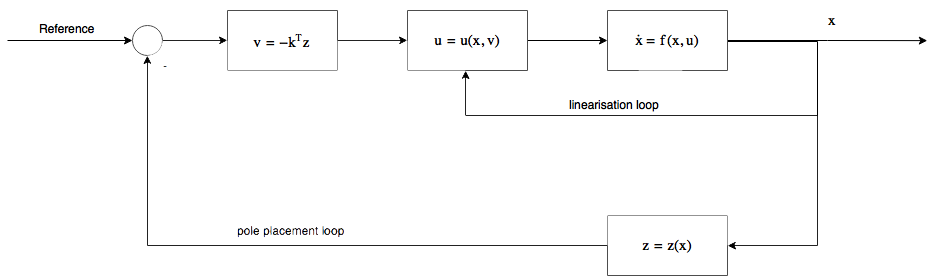
\includegraphics[width=1\textwidth]{Figures/NLI}
  \caption[Feedback linearisation example]{Feedback linearisation example \cite{Slotine+Li}}
  \label{fig:nli}
\end{figure}

EXPLAIN NECESSARY MATHEMATICAL CONCEPTS HERE

\subsection{SISO systems}
\label{section:background/SISO_NLI}

Although an aircraft is always considered as a MIMO system, a description of this control concept will firstly be provided for a general SISO case, before generalising to a MIMO case. Nonlinear systems that can be represented as $\dot{x}=f(x)+g(x)u$ will be discussed in this section. From \cite{Slotine+Li}, a definition of Input-State linearisation is to find, for a nonlinear system of relative degree $n$, a \emph{diffeomorphism} $\phi:\Omega \rightarrow R^n$ and nonlinear control law
\begin{equation}
u=\alpha(x) + \beta(x)\upsilon
\label{eq:nli_control_law}
\end{equation}

such that the new state variables $z=\phi(x)$ and \emph{pseudo-input} $\upsilon$ satisfy the linear time invariant system $\dot{z} = Az+B\upsilon$, where the following equations are satisfied

\begin{equation}
	\begin{cases}
		\dot{z_i}=z_{i+1} & if\quad i<n-1\\
		\dot{z_n}=\upsilon & if\quad i=n-1
	\end{cases}
	\label{eq:SISO_state}
\end{equation}

In order to find such a function and control law, one must find a state $z_1$ such that 
\begin{subequations}
	\begin{equation}
		\nabla z_1 ad_f^ig=0 \qquad i=0, ..., n-2
	\end{equation}
	\begin{equation}
		\nabla z_1 ad_f^{n-1}g\neq 0
	\end{equation}
\end{subequations}

The remaining states are then obtained from $z(x) = [z_1 \quad L_fz_1 \quad ... \quad L_f^{n-1}z_1]^T$ and the input transformation from

\begin{subequations}
	\begin{equation}
		\alpha (x) = - \dfrac{L_f^nz_1}{L_gL_f^{n-1}z_1}
	\end{equation}
	\begin{equation}
		\beta (x) = \dfrac{1}{L_gL_f^{n-1}z_1}
	\end{equation}
\end{subequations}

\subsection{MIMO systems}
\label{section:background/MIMO_NLI}

These concepts can also be extended to to MIMO systems in a similar manner, by similarly differentiating the outputs until the inputs explicitly appear. This time however, there are individual relative degrees per output. The sum of these relative degrees is called total degree $r$ and must satisfy $r<n$, $n$ being the order of the system. Given a MIMO system 
\begin{gather}
\dot{x} = f(x) + G(x)u\\
y=h(x)
\end{gather}
the $\phi$ functions are defined as $\phi^i_j(x)=L^{j-1}_fh_i(
x)$ and satisfy a condition similar to \ref{eq:SISO_state} 
\begin{equation}
\dot{\phi}^i_1(x)=\phi^i_2,...,\dot{\phi}^i_{r_i-1}=\phi^i_{r_i} \quad \text{and} \quad \dot{\phi}^i_{r_i}=L_f^{r_i}h_i(x)+\sum^m_{j=1}L_{g_j}L^{r_i-1}_fh_i(x)u_j
\end{equation}
As this equation holds for $1<i<p$, $p$ being the number of outputs of the system, giving an expression for the pseudo control input $\upsilon$
\begin{equation}
\upsilon = 
\begin{bmatrix}
\dot{\phi}^1_{r_1}\\
\vdots\\
\dot{\phi}^p_{r_p}\\
\end{bmatrix}
\end{equation}

It is also interesting to note the resulting system is not only linear, but also completely decoupled, as each new pseudo input only affects one output.

\section{Limitations of feedback linearisation}
\label{section:background/limitations}
Although feedback control answers to many of the problems of linear controllers such as PID and LQR, it has a big downside. Indeed, being a model based controller, it requires the system model to be quite accurately known. Let $\upsilon$ be the vector of pseudo inputs, for a second order $\ddot{x} = f(x,\dot{x},u)$, if it is input-output linearisable and the exact system is known, then it comes that, from \cite{YANG+LIN_Adaptive_Flight_Control}
\begin{equation}
\ddot{x}=\upsilon
\end{equation}
However, even for simpler models, a real system is difficult to accurately describe, and an approximation $\hat{f}$ of $f$ is usually chosen, resulting in $\upsilon=\hat{f}(x,\dot{x},u)$. Therefore, defining a dynamic inversion error, $\Delta(x,\dot{x},u)=f(x,\dot{x},u)-\hat{f}(x,\dot{x},u)$, comes that, as stated in \cite{YANG+LIN_Adaptive_Flight_Control}
\begin{equation}
\ddot{x}=\upsilon + \Delta(x,\dot{x},u)
\label{eq:system+error}
\end{equation}
There can be many causes for a dynamic inversion error to be present, as not only modelling incertitudes can lead to larger errors, but also external interference (wind gusts) and actuator faults. The goal of this section will be to present the reader with some solutions to minimize this error. 

\subsection{Fuzzy Logic Systems}
\label{section:background/fuzzy_logic}

Fuzzy logic systems are based on the paradigm of continuous levels of truth between 0 and 1, rather than the usual discrete true or false levels of truth. Using these continuous truth values, a set of IF-ELSE rules is chosen. The goal of this type of controller is to duplicate the way a pilot would respond to a given flight situation. These rules can base their control input based on variables such as roll, angle of attack and sideslip \cite{Comparison_IntelligentSys}. This control method is based on three main parts. The first one if \textit{fuzzification}, that consists of converting the plant outputs to fuzzy logic values. \textit{Rule-based inference}, using the previously mentioned set of rules, a fuzzyfied control input is computed, which then goes through the \textit{defuzzyfication} part of the control algorithm. 
Fuzzy systems have some advantages: its linguistic interpretation of human knowledge facilitate the interpretation of results, and the knowledge base can be improved through addition of new rules. However, this method comes with some disadvantages. First of all, the set of rules that will will improve the control of the aircraft is entirely dependent on expert knowledge, thus resulting in an empiric set of rules. This also means the method has no capability of generalization, as the control is only applied to specific cases, of the form "if the error is greater than a given value, apply this compensation to control input". It is also not robust to topological changes of the system \cite{Neuro_fuzzy_survey}. For these reasons this method will not be further studied and implemented in this work.


\subsection{Neural Networks}
\label{section:background/NN}

Artificial Neural Networks (NN) are a biologically inspired simulation of brain's nervous system. They are composed of simulated neurons and synapses. The sum of the inputs of a neuron are summed and the result is fed into an activation function, which then return a bounded value, either between -1 and 1 or 0 and 1. The inputs and outputs of a neuron are multiplied by a weight, representing the synapses between neurons. We get the following equation for one neuron
\begin{equation}
y(x_1,x_2,...,x_n)=f((\sum ^n_{i=1} w_i x_i)+b)
\end{equation}
where $b$ is the bias term and $f$ a given activation function. Neuron are then set in three different types of layers: the input, the output and the hidden layers. These are connected between each other, and the hidden part can be composed of several layers. The weights can then be tuned based on experience, making it suitable for intelligent learning. To tune these weights learning algorithms are used. There are two types of learning algorithms: batch and online training. It is called training to the process of iteratively reaching the ideal set of weights that will minimise the error between the output of the neural network and that of a given unknown function.

Batch training is mostly based one a property NN is that, according to the Universal Approximation Theorem showed in 1989 by George Cybenko, a feed forward neural network can approximate any continuous function. The network is trained by providing input and output pairs. The weights are found in order to approximate the output of the neural network to that of the original function. Once these weights are computed, the network can then be used to compute outputs from inputs that were not part of the initial knowledge of input-output pairs.

Although this learning method approach is used in many of NN applications, it cannot however be easily used to improve an existing feedback linearisation  controller, as it requires an \textit{a priori} knowledge of the modelling error for each given input.

Online training, contrary to batch training, can deal with dynamically changing environments. This training paradigm is not based on an \textit{a priori} knowledge set, and instead relies on update laws that compute the new weights after each control iteration. It is this method that will be retained to adaptively correct the inversion error from the feedback linearisation. Training a network online, however, is less trivial when compared to batch training. An algorithm named backpropagation will be presented to provide a way of training a network online.  


%Backprop
The backpropagation algorithm is one of the most common NN training algorithm, commonly used in batch training, used to update the weights of each layer of a network, in order to minimize a cost function. However, research has been done in order to use backpropagation techniques to create online adaptive and augmented control such as \cite{online_adaptiveNN}, \cite{UAV_adaptive}, \cite{UAV_adaptive2}. Indeed, it is also possible to use such algorithms to continuously update the weights of a network as the data is generated. Backpropagation can only be implemented if the activation function of the NN is differentiable. 

The backpropagation algorithm can be described by a two phase cycle, Propagation and Weight update. During this last phase the gradient descent algorithm is used to optimize a cost function. As such, a cost function $E$ must be chosen, and must be a function of the outputs of the neural network. A commonly used error function is 
\begin{equation}
E=\frac{1}{2} (y_d-y)^2
\end{equation}

Where $y_d$ is the desired output of the network and $y$ is the actual output of the network. The $\frac{1}{2}$ factor is added to be cancelled when differentiating. For a given neuron $i$, the sum of its inputs $sum_i$ is given by
\begin{equation}\label{eq:def_sum}
sum_i = \sum ^n_{k=1} w_{ki} x_k
\end{equation}
Where $w_{ki}$ is the weight of the $k^{th}$ input of neuron $i$, and $x_k$ are the outputs of the neurons form the previous layer. Given an activation function $f(x)$, we define the output of neuron $i$ as 
\begin{equation}\label{eq:NN_output}
x_i = f(sum_i)
\end{equation}

In order to use the gradient descent algorithm, the derivative of the cost function with respect to a given weight $w_{ij}$ must be computed. To do so, the chain rule is used as such
\begin{equation}\label{eq:gradient}
\frac{\partial E}{\partial w_{ij}} = \frac{\partial E}{\partial x_j}\frac{\partial x_j}{\partial sum_j}\frac{\partial sum_j}{\partial w_{ij}}
\end{equation}
These three factors can now be easily computed. The last two factors are independent of weather $x_j$ is a hidden or output layer and will for this reason be calculated firstly. From \ref{eq:def_sum} and \ref{eq:NN_output} comes that
\begin{equation}
\frac{\partial x_j}{\partial sum_j} = \frac{\partial f(sum_j)}{\partial sum_j}
\end{equation}
For an output layer, where values may be unbounded, linear output functions may be used, for which the equation above has a trivial solution. For output layers of classification neural networks or for hidden layers in general, logistic or tangent sigmoid functions can be used instead. For the first case let $f(x)=\frac{1}{1+e^{-x}}$, then

\begin{equation}
\frac{\partial f(sum_j)}{\partial sum_j}=f(sum_j)(1-f(sum_j))
\end{equation}
For the case of a tangent sigmoid activation function $f(x)=tanh(x)$ comes
\begin{equation}
\frac{\partial f(sum_j)}{\partial sum_j}=1-f^2(sum_j)
\end{equation}

For the term $\frac{\partial sum_j}{\partial w_{ij}}$, from \ref{eq:def_sum} this partial derivative is easily computed

\begin{equation}
\frac{\partial sum_j}{\partial w_{ij}} = \frac{\partial \left(\sum ^n_{k=1} w_{kj} x_k\right)}{\partial w_{ij}} = x_i
\end{equation}

For the output layer, the first term of equation \ref{eq:gradient} can easily be evaluated, as $x_j=y$ for such a case, giving
\begin{equation}
\frac{\partial E}{\partial x_j}=\frac{\partial (\frac{1}{2} (y_d-y)^2)}{\partial y}= y-y_d
\end{equation}
For input layers however, this derivative is less obvious to estimate. One can consider that the error function $E$ is a function of the inputs of all neurons that take $x_j$ as input. Let $S$ be such a set of inputs, from the total derivative to $x_j$ comes that
\begin{equation}
\frac{\partial E}{\partial x_j} = \sum _{s\in S}\left( \frac{\partial E}{\partial x_s}\frac{\partial x_s}{\partial sum_s}\frac{\partial sum_s}{\partial x_j}\right)=\sum _{s\in S}\left( \frac{\partial E}{\partial x_s}\frac{\partial f(sum_s)}{\partial sum_s}w_{js}\right)
\end{equation}
Note that the term $ \frac{\partial E}{\partial x_s} $ represent the all the derivatives of the errors with respect to the outputs of the next layer of neurons. Taking into account that the last layer is easily evaluated without this method, the derivatives of all hidden neurons can be computed. Knowing the value of \ref{eq:gradient}, an update law for the weights can now be stated from the gradient descent algorithm
\begin{equation}\label{eq:update_law}
\Delta w_{ij} = - \alpha \frac{\partial E}{\partial w_{ij}}
\end{equation}
Where $\alpha$ is a learning coefficient, and its choice is crucial to assure a fast convergence of the solution. Indeed, while a exceedingly large learning coefficient can cause this algorithm to miss the minimum error, a small learning coefficient will also increase the convergence rate. The $-1$ factor is added in the equation above to converge to a local minima, removing it would make this algorithm maximize the cost function. A limitation of the backstepping algorithm that must also be taken into account is that it only guarantees local minima convergence. 

